\section{Discrete Wavelet Transform (DWT) decomposition}
In \cite{citeulike:3734066} Popivanov and Miller discussing the time-series similarity search using wavelets-based dimensionality reduction. In this work they are exploring further away from previously used Haar wavelets \cite{citeulike:4384535} and showing that some of the wavelets outperform not only Haar wavelets but also the best-known non-wavelet approaches for the time-series similarity up to date (DFT, DCT, SVD etc.). Their approach for time series approximation benefits from such a wavelet-transform properties as:
\begin{itemize}
	\item{Compact support: there are flavors of the wavelet transform such that a basis function is non-zero only at the finite interval, which allows wavelet approximation to capture local time-series features as opposite to DFT based approach which is capturing only global features.}
	\item{Efficiency: while FFT complexity is $O(n \log{n}$, wavelet transform is linear to the size of the data and is real-to-real transform.}
	\item{Sensitivity: wavelet transform allows fine tuning of the approximation by selecting the different scales, corresponding to basis functions of different length where the DFT gives.}
\end{itemize}

The wavelet is a function, $\psi_{j,k}$ defined on $\mathbb{R}$ with shift $k$ and dyadic dilation (a product of power of $2$, referred as stretching). The set of functions defined as
\begin{equation}
\psi_{j,k} = 2^{j/2} \psi \left( 2^{j}t - k \right)  
\label{eq:wavelet}
\end{equation} 
for $j, k \in \mathbb{Z}$ form a complete orthonormal system over $L^{2}(\mathbb{R})$ and can be used to define any signal $f \in L^{2}(\mathbb{R})$ uniquely by the following series: 
\begin{equation}
f = \sum_{j, k \in \mathbb{Z}} \left\langle f, \psi_{j,k} \right\rangle  \psi_{j,k}, \\
\text{where} \left\langle f,g \right\rangle = \int_{\mathbb{R}} f g \: dx \; \text{, the inner product}
\label{eq:wavelet_series}
\end{equation} 
The function $\psi_{j,k}$ is the ``basis function'' of the wavelet (mother wavelet function) and essentially wavelet can use an infinite family of basis functions as opposite to Fourier transform which uses only exponential function. 
\begin{figure}[tbp]
   \centering
   \includegraphics[height=65mm]{dwt.eps}
   %%{seriesheatmap}
   \caption{The combination of figures from \cite{citeulike:3734066} illustrating an advantage of Daubechies wavelet over the Haar wavelet (a, b, c, d, f) and other methods (e) such as DFT and PAA.}
   \label{fig:dwt}
\end{figure} 

It has been proven \cite{citeulike:499150} that the energy of the wavelet features lies between two non-negative bounds:
\begin{equation}
A \left\| X \right\|^{2} \leq \left\| x \right\|^{2} \leq B \left\| X \right\|^{2}
\label{eq:dwt_bounds}
\end{equation}
where $A$ and $B$ are non-negative constants, $x$ is the signal and $X$ it's wavelet transform $X=T(x)$. 

For the $\epsilon$-radius range query and equation \ref{eq:dwt_bounds} we have the following inequality:
\begin{equation}
A \left\| X-Q \right\|^{2} \leq \left\| x-q \right\|^{2} < \epsilon^{2} 
\label{eq:}
\end{equation}
which provides us with the confidence of no false-dismissals (lower bounding property).

Popivanov \& Miller along with Chan \& Fu \cite{citeulike:4384535} proved the superiority of DWT over Fourier transform, SVD and PAA methods in both, the speed of index building and the precision of the range-query processing while using the same F-index and $R^{*}$-tree as in the previous time-series similarity work.  